\documentclass[svgnames,11pt]{beamer}
\input{/home/tof/Documents/Cozy/latex-include/preambule_commun.tex}
\input{/home/tof/Documents/Cozy/latex-include/preambule_beamer.tex}
%\usepackage{pgfpages} \setbeameroption{show notes on second screen=left}
\author[]{Christophe Viroulaud}
\title{Andy Warhol}
\date{\framebox{\textbf{Lang 07}}}
%\logo{}
\institute{Première - NSI}

\begin{document}
\begin{frame}
    \titlepage
\end{frame}
\begin{frame}
    \frametitle{}

    Artiste américain mort en 1987, Andy Warhol était un  des principaux représentants du \emph{pop art}.	Le \emph{dyptique de Marylin Monroe} réalisé en 1962 est une de ses œuvres célèbres. Il contient cinquante fois la même image de l'actrice mais avec un travail des couleurs différent.
    \begin{center}
        \centering
        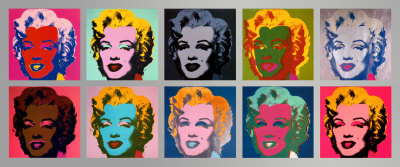
\includegraphics[width=8cm]{ressources/marylin.jpg}
        \captionof{figure}{Dyptique de Marylin Monroe}
        \label{IMG}
    \end{center}
    \note{\fcolorbox{black}{red}{{\LARGE warhol.zip sur site}}}
\end{frame}
\begin{frame}
    \frametitle{}

    \begin{framed}\centering
        Comment réaliser une reproduction du concept de cette œuvre?
    \end{framed}

\end{frame}
\section{Manipuler une image}
\subsection{Présentation de la bibliothèque}
\begin{frame}[fragile]
    \frametitle{Présentation de la bibliothèque \textbf{\texttt{Pillow}}}
    La bibliothèque \texttt{\textbf{Pillow}} (nouvellement nommée \textbf{\texttt{PIL}}) est un outil pour faciliter la manipulation des images.
    
\end{frame}
\begin{frame}[fragile]
    \frametitle{}

    \begin{center}
        \begin{lstlisting}[language=Python , basicstyle=\ttfamily\small, xleftmargin=2em, xrightmargin=2em]
from PIL import Image

originale = Image.open("joconde.jpg")
ligne, colonne = originale.size
\end{lstlisting}
        \captionof{code}{La bibliothèque \textbf{\texttt{Pillow}}}
        \label{pil}
    \end{center}
    \begin{activite}
        \begin{enumerate}
            \item Lire et tenter de comprendre le rôle de chaque ligne du code \ref{pil}.
            \item Télécharger et extraire le dossier compressé \textbf{\texttt{warhol.zip}} sur le site \url{https://cviroulaud.github.io}.
            \item Copier le code \ref{pil} dans un fichier \textbf{\texttt{warhol.py}}.
        \end{enumerate}
    \end{activite}

\end{frame}
\begin{frame}
    \frametitle{Avant de regarder la correction}
    \begin{center}
        \centering
        \includegraphics[width=3cm]{/home/tof/Documents/Cozy/latex-include/stop.png}
    \end{center}
    {\Large
    \begin{itemize}
        \item Prendre le temps de réfléchir,
        \item Analyser les messages d'erreur,
        \item Demander au professeur.
    \end{itemize}
    }
\end{frame}
\begin{frame}[fragile]
    \frametitle{Correction}

    \begin{center}
        \begin{lstlisting}[language=Python , basicstyle=\ttfamily\small, xleftmargin=2em, xrightmargin=2em]
# Import de l'outil 'image' de la bibliothèque Pillow
from PIL import Image

# Affectation de l'image 'joconde' à la variable 'originale'
originale = Image.open("joconde.jpg")

# Récupération des dimensions de l'image
ligne, colonne = originale.size
\end{lstlisting}
        \captionof{code}{La bibliothèque \textbf{\texttt{Pillow}}}
    \end{center}

\end{frame}
\subsection{Couleurs d'une image}

\begin{frame}
    \frametitle{Couleurs d'une image}

    Une image peut être vue comme un tableau de pixels de \textbf{\texttt{l}} lignes et \textbf{\texttt{c}} colonnes. Chacun de ces points de l'image code une couleur.
    \begin{center}
        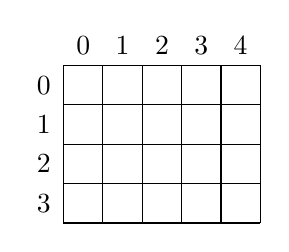
\begin{tikzpicture}[scale=0.5]
            \draw (0,0) grid (5,4);

            \draw (-0.5,3.5) node{0};
            \draw (-0.5,2.5) node{1};
            \draw (-0.5,1.5) node{2};
            \draw (-0.5,0.5) node{3};
            \draw (0.5,4.5) node{0};
            \draw (1.5,4.5) node{1};
            \draw (2.5,4.5) node{2};
            \draw (3.5,4.5) node{3};
            \draw (4.5,4.5) node{4};
        \end{tikzpicture}
        \captionof{figure}{Coordonnées d'un pixel}
    \end{center}
\end{frame}
\begin{frame}
    \frametitle{}

    Pour obtenir une grande gamme de couleurs, le principe de la synthèse additive est utilisé. En combinant une quantité de Rouge, Vert, Bleu (RGB en anglais) il est possible de créer une palette importante.
    \begin{center}
        \centering
        
\includegraphics[width=5cm]{ressources/additive.jpg}
        \captionof{figure}{Synthèse additive}
        \label{IMG}
    \end{center}
    Chaque pixel peut ainsi être vu comme une superposition (Rouge, Vert, Bleu); chaque composante étant codé sur \textbf{1 octet}.
\end{frame}
\begin{frame}
    \frametitle{}

    \begin{activite}
        Sachant qu'un \textbf{octet} peut prendre 256 valeurs, calculer le nombre de couleurs qu'il est possible de composer en mélangeant le rouge, le vert et le bleu.
    \end{activite}

\end{frame}
\begin{frame}
    \frametitle{Avant de regarder la correction}
\begin{center}
    \centering
    \includegraphics[width=3cm]{/home/tof/Documents/Cozy/latex-include/stop.png}
    \end{center}
{\Large
    \begin{itemize}
        \item Prendre le temps de réfléchir,
        \item Analyser les messages d'erreur,
        \item Demander au professeur.
    \end{itemize}
}
\end{frame}
\begin{frame}
    \frametitle{Correction}

    \begin{itemize}
        \item Il y a 256 rouges, 256 verts, 256 bleus.
        \item On peut composer
        $$256×256×256=16777216$$ couleurs
    \end{itemize}

\end{frame}
\subsection{Principe de la modification}
\begin{frame}
    \frametitle{Principe de la modification}

    

\end{frame}
\end{document}